\documentclass{article}
\usepackage[utf8]{inputenc}
\usepackage[spanish]{babel}
\usepackage{listings}
\usepackage{graphicx}
\graphicspath{ {images/} }
\usepackage{cite}

\begin{document}

\begin{titlepage}
    \begin{center}
        \vspace*{1cm}
            
        \Huge
        \textbf{Taller Memoria}
            
        \vspace{0.5cm}
        \LARGE
        Trabajo de investigación.
            
        \vspace{1.5cm}
            
        \textbf{Juan Camilo Mazo Castro}
            
        \vfill
            
        \vspace{0.8cm}
            
        \Large
        Despartamento de Ingeniería Electrónica y Telecomunicaciones\\
        Universidad de Antioquia\\
        Medellín\\
        Septiembre de 2020
            
    \end{center}
\end{titlepage}

\tableofcontents

\section{Introducción}
En el presente trabajo se hace con el fin de entender mejor el funcionamiento y la gestión que se le da a la memoria de un computador, esta información será fundamental para poder entender algunos conceptos y conocimientos necesarios que debe tener un programador. Se resolverán una serie de preguntas planteadas con respecto al tema comentado anteriormente.

\section{Sección de contenido} \label{contenido}

1.Defina qué es la memoria de un computador.

Una memoria es un dispositivo electrónico que sirve para almacenar información ya sea temporal o permanentemente. Normalmente se utiliza el termino memoria para referirse a dispositivos de almacenamiento temporal y de alta velocidad de acceso como la memoria RAM o las memorias Cache incluidas en algunos procesadores, sin embargo, también hay otras de almacenamiento permanente como los discos duros.
Las memorias cumplen un papel muy importante en el funcionamiento de las maquinas. Éstas junto con otros dispositivos permiten que puedan funcionar correctamente todos los programas que utilizamos hoy en día, permiten que se almacene y se procese toda la información que solicitamos y requerimos. Las memorias tienen una capacidad de almacenamiento de la información mucho más grande que otros dispositivos, por lo que se hacen indispensables para que nuestras computadoras funcionen. Para lograr el objetivo antes dicho, los diferentes tipos de memoria trabajan en equipo junto con otros dispositivos como el microprocesador y los controladores.

2.Mencione los tipos de memoria que conoce y haga una pequeña descripción de cada tipo.

Disco Duro: Tiene una gran capacidad de almacenamiento y funciona con unos discos que giran, es más lenta para dar acceso a la información por lo que es utilizada para almacenar datos que se quieren guardar permanentemente. Es muy importante pues guarda información que se requiere para que el usuario pueda hacer uso de la computadora, los datos necesarios para efectuar cualquier programa se toman de esta y se ponen en la memoria RAM para que el microprocesador tenga un acceso más rápido a ellos. Además, el Disco Duro guardará permanentemente todas las modificaciones que se le hagan a los archivos que tiene el usuario cuando el desee guardarlos.

Memoria Virtual: Es una parte del Disco Duro que se utiliza para guardar datos que ocupan una buena parte de almacenamiento y que no se utilizan tanto, pero que de igual forma se mantienen ahí para que se puedan utilizar cuando sean requeridos y mientras se encuentran en la Memoria Virtual no ocupan espacio innecesario en la memoria RAM.\cite{YouBioit}

Memoria RAM: es una memoria de almacenamiento temporal que es de gran ayuda para el microprocesador, mientras se ejecuta un programa esta almacena los datos temporales que el microprocesador va requiriendo a medida que ejecuta las ordenes que se le demandan. Tiene menor capacidad de almacenamiento y da acceso a la información más rápido que un Disco Duro. La memoria RAM almacena también las ordenes que se le solicitan al microprocesador para que este las pueda leer y ejecutar.
 
Memoria Cache: Es una memoria de menor capacidad que la memoria RAM, se encuentra en algunos procesadores como los Intel Core i5 y al encontrarse en el mismo procesador, tiene un acceso más rápido a la información que estas guardan. Existen tres tipos de Caché diferentes, la L1, L2 y L3. L1 es la más veloz y es la que tiene menor almacenamiento de las tres,L2 es un punto intermedio entre L1 Y L3, L3 tiene el mayor almacenamiento de las tres pero es menos veloz que L1 Y L2, aun así sigue siendo más veloz que la memoria RAM. Se utiliza para almacenar datos que se utilizan con mayor frecuencia por el usuario, así le evita al procesador tener que retirar la información de la memoria RAM que es más lenta.\cite{YouBioit}

Memoria USB: Es una memoria portable de almacenamiento permanente, no tienen demasiado espacio de almacenamiento, pero sirven para guardar datos de un computador y utilizarlos en otro.

Memoria ROM: Es una memoria no volátil que se encuentra en la placa madre de los computadores, esta le da las primeras instrucciones al microprocesador cuando la maquina se enciende.

DRAM: Es un tipo de memoria volátil, es decir que cuando se le corta la corriente eléctrica los datos en ella desaparecen. Se le llama Dynamic RAM porque cada cierto tiempo necesita un ciclo de refresco de datos para que estos permanezcan.

Las memorias también se pueden dividir en dos tipos, memorias volátiles que no almacenan la información de manera permanente y las no volátiles que por el contrario sí lo hacen. Algunos ejemplos se muestran el la figura 1. (\ref{fig:Volatilidad})

\begin{figure}[h]
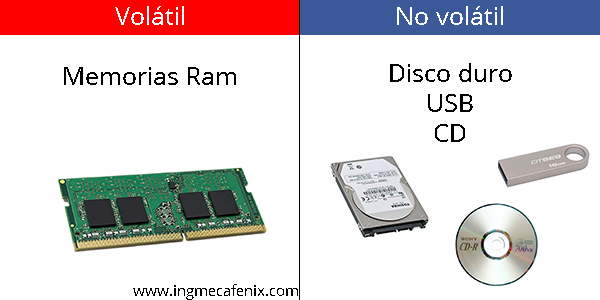
\includegraphics[width=6cm]{Volatilidad.jpg}
\centering
\caption{Ejemplos memorias volatiles y no volatiles}
\label{fig:Volatilidad}
\end{figure}


3.Describa la manera en que se gestiona la memoria en el computador.

Cuando nuestras computadoras se encienden lo primero que hace el procesador es esperar que se le indiquen las primeras instrucciones, estas las tiene la memoria ROM que guarda de manera permanente las instrucciones que se deben realizar siempre que empieza a trabajar la máquina. Una vez la memoria RAM ya se encuentra en funcionamiento lo primero que hace es cargar la BIOS que contiene información del sistema operativo que se encuentra en el Disco Duro de arranque, así una vez iniciado el sistema operativo el usuario puede empezar a utilizar la computadora. Ya en este punto el usuario empieza a efectuar ciertas ordenes que le dan instrucciones al procesador, el procesador utiliza la memoria RAM para guardar y tener un acceso más rápido a los datos que el usuario requiere para que funcionen los programas que él necesita. Los controladores de memoria hacen un espacio en la memoria RAM para traer del Disco Duro los datos requeridos, una vez en la RAM el procesador hace uso de ellos y cuando ya no los necesita, si tienen modificaciones y el usuario desea guardarlos, el Disco Duro se encarga de guardarlos permanentemente. La memoria RAM siempre carga todos los datos necesarios para que los programas que utilizamos puedan funcionar, cuando los datos son demasiado grandes y la memoria RAM no puede con todos ellos se hace uso de la memoria virtual, pero cuando se hace esto el computador empieza a funcionar de una forma más lenta, pues el procesador tarda más en tener acceso a los datos que se encuentran ahí. Además de la memoria RAM también se cuenta con la memoria Cache que se encuentra en el procesador, esta almacena información que se usa con más recurrencia para que cada vez que el procesador requiera esos datos para ejecutar un programa tenga un acceso más rápido a ellos. En conclusión, la memoria RAM sirve como apoyo para el microprocesador, le ayuda a cargar toda la información que este no puede almacenar por si solo, información que este requiere para efectuar los procesos de las ordenes que se le indican.  La gestión que se le da a cada una de las memorias se hace con el objetivo de tener una mayor eficiencia en la ejecución de los diferentes trabajos que hace la máquina.\cite{YouBioit}


4.¿Qué hace que una memoria sea más rápida que otra?¿Por qué es tan importante?

La velocidad de una memoria puede depender de la manera en que lee los datos, ya sea con un patrón secuencial o con un patrón aleatorio. Por ejemplo, un disco duro SSD SATA lll con patrones aleatorios da acceso a los datos más rápido que un disco duro de 5400 rpm que tiene un patrón secuencial.
Otro factor que hace que una memoria sea más rápida que otra es la latencia, es decir el tiempo que se espera para recibir el primer dato desde una memoria. En los discos duros, el tiempo de la latencia es del orden de los milisegundos y en las memorias RAM, es del orden de los nanosegundos.
Por otro lado, se puede tener en cuenta la cantidad de almacenamiento que tiene una memoria, pues usualmente cuando un dispositivo tiene más capacidad de almacenamiento, tiene menor velocidad. Cuando una memoria es no volátil suele tener más espacio para almacenar, esta guarda los datos permanentemente, por otro lado, una memoria que es volátil solo almacena la información mientras tenga corriente y tiene un menor espacio de almacenamiento. Las memorias volátiles, como la memoria RAM por ejemplo, suelen usarse para almacenar temporalmente datos que son necesarios mientras se ejecuta alguna instrucción en nuestro computador, estas suelen ser más rápidas que una memoria no volátil, como el disco duro, que guarda de manera permanente los archivos que no son requeridos en el momento.
La importancia de una memoria más rápida es la eficiencia y la fluidez con la que funcionan nuestras computadoras y las tareas que se llevan a cabo en estas. Además, ciertos dispositivos funcionan con ayuda de la memoria en nuestros computadores como los procesadores o  los controladores de la placa madre, un procesador que trabaja a una gran velocidad requiere de un soporte como la memoria RAM que pueda seguirle el ritmo.\cite{Alelua}


En la figura número dos se muestra la jerarquía desde la memoria con mayor velocidad a la que tiene menor velocidad y desde la que tiene menor almacenamiento a la que mayor almacenamiento tiene. (\ref{fig:jerarquia})

\begin{figure}[h]
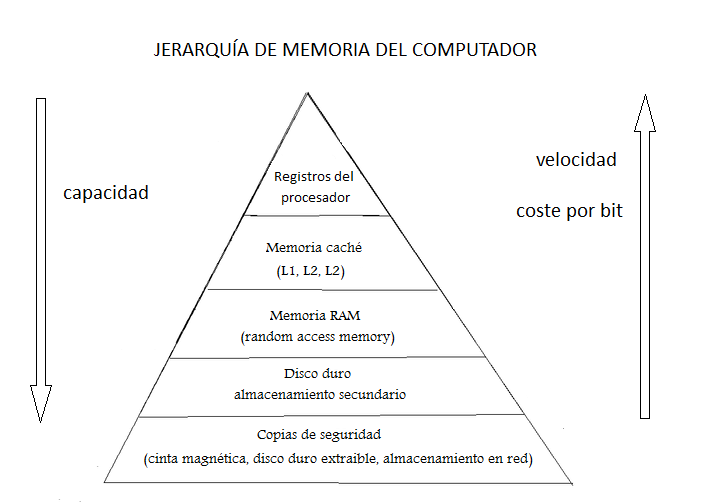
\includegraphics[width=8cm]{jerarquia.png}
\centering
\caption{Jerarquía memorias}
\label{fig:jerarquia}
\end{figure}


\section{Conclusión} \label{conclulsion}

Las memorias son sumamente importantes por la capacidad de almacenamiento que poseen, la disponibilidad de espacio para guardar información que brindan debe ser aprovechada al máximo para poder tener una mejor eficiencia con los recursos de nuestras maquinas.

Cuando se llena de demasiados datos a un dispositivo que almacena información como un Disco Duro, el tiempo que tarda extraer uno de esos datos almacenados se hace más grande. Esto también puede ocurrir con la Memoria RAM, si esta es saturada de información, recurre a la memoria virtual haciendo que la velocidad del ordenador en general disminuya. Por esto es que es importante saber aprovechar al máximo el espacio en el que vamos a guardar los datos que vamos a requerir para ejecutar un programa cuando estamos programando, hay que encontrar la manera en que solo se almacenan los datos que son absolutamente necesarios y se eliminan los que no son requeridos, el rendimiento de nuestros programas aumentará en gran medida si tenemos esto en cuenta. 


\bibliographystyle{IEEEtran}
\bibliography{references}

\end{document}
